% !TEX encoding = UTF-8 Unicode
\chapter{Metodología propuesta}
\label{chap:propuesta}
%
%
En este capítulo se establecerá y detallará la propuesta para realizar un acomodo de objetos, con la condición de minimizar el número de acciones que conlleva el acceder a cada uno de ellos.
Dicha propuesta se basa en un sistema de puntuaciones, asignadas a cada uno de los elementos en la malla incluyendo celdas vacías.
La puntuación que se asignará a cada elemento dependerá de la clase del elemento en cuestión así como de su vecindad.

La puntuación de un elemento, cuando se trate de un objeto, será máxima cuando este se pueda tomar mediante una sola acción y disminuye con la presencia de vecinos que impiden su agarre o sujeción.
En el caso de las celdas vacías, su puntuación se incrementa con respecto al número de celdas vecinas que sean ocupadas por objetos, y disminuye en función del número de celdas vecinas vacías.

Con este sistema de puntuaciones, el cual es parte fundamental de las aportaciones de la propuesta aquí presentada, se busca que la puntuación global de la malla, esto es, la suma de las puntuaciones de los elementos individuales, sea máxima; lo cual es sinónimo de un fácil acceso y posterior sujeción de los objetos.

Los procesos para calcular las puntuaciones mencionadas son integrados en una función, la cual es a su vez utilizada por un algoritmo de recocido simulado, en el cual convergen las aportaciones de este trabajo y que se encarga de hacer los cambios necesarios a un acomodo inicial aleatorio, con la finalidad de que la puntuación global se maximice.
De esta forma es como se obtendrá un acomodo de objetos optimizado para realizar el acceso y la sujeción de cada uno de los objetos en una malla, con un número de acciones mínimas en promedio, lo cual en la práctica también podría implicar un tiempo mínimo promedio para acceder a los objetos.
Para ello se evalúan los acomodos obtenidos por el algoritmo al calcular el costo de tomar cada objeto de la malla mediante una función de costo.

La definición completa del algoritmo y de las funciones mencionadas se dará en las siguientes secciones.
%
%
\section{Funciones y procedimientos propuestos}
\label{sec:funciones_y_procedimientos}
%
%
En esta sección se iniciará con la definición de los componentes más básicos de la metodología propuesta, posteriormente se definirán las funciones y procedimientos de más alto nivel, que hacen uso de dichos componentes y finalmente, en la Sección \ref{sec:algoritmo_principal}, se describirá el algoritmo principal de la propuesta, el cual es la definición de más alto nivel de esta.

Con la finalidad de simplificar la notación de algunos cálculos posteriores, se define $C_0$ como la clase de una celda vacía, la cual, al solo tener fines de representación, no tiene ningún atributo asociado.
Asimismo se define $h_{ij}$ como la altura del elemento en la celda $e_{ij}$, definiendo la altura de una celda vacía como cero.

Se define la función de estado $C_{ij}$ como la función que retorna la clase del elemento posicionado en la celda $e_{ij}$.
%
\begin{equation}
	C_{ij} \mapsto C \cup \{ C_0 \}
\end{equation}
%
Además, se define la función de sujeción $S_{ij}$ como la función que retorna el subconjunto de formas de sujeción permitidas de un objeto posicionado en la celda $e_{ij}$.
%
\begin{equation}
	S_{ij} \mapsto S'_K \hspace{1pt}, \qquad S'_K \subseteq S_K
\end{equation}
%
Las expresiones que describen las condiciones bajo las cuales los objetos pueden ser sujetados, correspondientes a la descripción dada en la Sección \ref{subsec:restricciones}, se presentan a continuación:
%	
\begin{equation}
\label{eq:restricciones}
	\begin{aligned}
		&h_{i+1,\, j} < h_{ij}\ \wedge\ h_{i-1,\, j} < h_{ij}\ \Rightarrow\ H \in S_{ij} \\[0.7em]
		&h_{i,\, j+1} < h_{ij}\ \wedge\ h_{i,\, j-1} < h_{ij}\ \Rightarrow\ V \in S_{ij}
	\end{aligned}
\end{equation}
%
Por lo tanto, la condición para que un objeto en una celda $e_{ij}$ sea sujetable es simplemente:
%
\begin{equation}
\label{eq:sujetable}
	|S_{ij}| \geq 1
\end{equation}
%
Con fines de legibilidad en definiciones posteriores, se utilizará la función booleana $\f{sujetable}(e_{ij})$, la cual simplemente indica si para el elemento de la celda $e_{ij}$ se cumple o no la condición de la Ecuación \ref{eq:sujetable}.
De forma similar, la función $\f{imposible}(e_{ij})$ indica si el elemento en la celda $e_{ij}$ pertenece a un cuadro imposible, como los que se describen en la Sección \ref{sec:casos_triviales_e_imposibles}.
%
%
\subsection{Funciones de ponderación}
\label{subsec:funciones_ponderacion}
%
%
A continuación se presenta la función que asigna una puntuación (un número entero) a un par de elementos vecinos en $E$.

Algo a tener en cuenta con esta función es que, si bien por si sola es una función que solo puntúa un par de elementos en la malla, está pensada para ser una sub-función del proceso de puntuación de más alto nivel de la Función \ref{func:puntuacion_elemento}, enfocado a puntuar un elemento particular de la malla en función de su vecindad.
Particularmente es el elemento del primer argumento de la Función \ref{func:puntuacion_par} el que será puntuado respecto a su vencindad en la Función \ref{func:puntuacion_elemento}.
Esta es una de las razones por las que en algunos casos el resultado de la función no sea conmutativo respecto al orden de sus argumentos, ya que en el proceso de puntuación de más alto nivel se le da más ``atención'' al primer argumento de la función, al ser considerado como el elemento a puntuar.
%
\begin{center}
\begin{minipage}{0.9\textwidth}
\begin{function}[H]
	\OneHalfBlankLine
	\Data{Celdas de los elementos vecinos $e_{i_1 j_1}$, $e_{i_2 j_2}$.}
	\Result{Puntuación.}
	\OneHalfBlankLine
	\Function{$\f{puntuacionPar}(e_{i_1 j_1}$, $e_{i_2 j_2})$}{
		\HalfBlankLine
		\Switch{$C_{i_1 j_1}$, $C_{i_2 j_2}$}{
			\HalfBlankLine
			\lCase{$C_1$, $C_0$}{\Return 3}
			\lCase{$C_1$, $C_2$}{\Return 1}
			\lCase{$C_2$, $C_1$}{\Return 2}
			\lCase{$C_2$, $C_0$}{\Return 1}
			\lCase{$C_0$, $C_1$}{\Return 2}
			\lCase{$C_0$, $C_2$}{\Return 1}
			\lCase{$C_{k_C}$, $C_{k_C}$}{\Return 0}
		}
	}
	\caption{puntuacionPar($e_{i_1 j_1}$, $e_{i_2 j_2}$). Función para obtener la puntuación de un par de elementos vecinos.}%
	\label{func:puntuacion_par}%
\end{function}
\end{minipage}
\end{center}
%
El sistema de puntuación presentado en la Función \ref{func:puntuacion_par} fue diseñado en base a heurísticas simples, esto con el propósito de que su implementación fuese eficiente en términos de velocidad de procesamiento.
Sin embargo, se intentó mantener un balance entre la eficiencia en el número de operaciones, proporcionada por la simpleza de las reglas de puntuación; y la eficiencia de los arreglos encontrados por el algoritmo, que está definida en términos del número total de acciones necesarias para tomar los objetos.

Dicho lo anterior, y teniendo en cuenta que posteriormente el primer argumento de la Función \ref{func:puntuacion_par} fungirá como el elemento a ser puntuado en la Función \ref{func:puntuacion_elemento}, las heurísticas detrás del sistema de puntuación utilizado en la Función \ref{func:puntuacion_par} son las siguientes:
%
\begin{itemize}
	\item Para los cubos (casos $C_1$, $C_0$ y $C_1$, $C_2$): la puntuación es máxima cuando su vecino es una celda vacía, debido a que es el elemento que puede permitir su sujeción; y es mínima, pero no cero, cuando su vecino es un prisma, ya que, si bien se restringe la sujeción del cubo, aún hay posibilidad de que el prisma sí pueda ser sujetable.
	\item Para los prismas (casos $C_2$, $C_1$ y $C_2$, $C_0$): la puntuación es máxima cuando su vecino es un cubo, pero no tanto como la del par \textsl{cubo-celda\,vacía}.
	La razón de esto es que, si bien la sujeción del prisma no se restringe, la del cubo sí, mientras que en el caso del par \textsl{cubo-celda\,vacía} no se genera ninguna restricción de sujeción.
	Por otro lado, la puntuación es mínima, pero no cero, cuando el vecino de un prisma es una celda vacía; esto debido a que, si bien la sujeción del prisma no se restringe, es posible que la celda vacía pueda ser mejor aprovechada al colocarla al lado de un cubo.
	\item Para las celdas vacías (casos $C_0$, $C_1$ y $C_0$, $C_2$): la puntuación es máxima cuando su vecino es un cubo, debido a que la celda vacía es el único elemento que permite su sujeción; y es mínima, pero no cero, cuando su vecino es un prisma, ya que permite su sujeción pero también existe otro elemento que la permite, pudiendo ser una mejor elección en determinadas situaciones.
	\item Para vecinos de la misma clase (caso $C_{k_C}$, $C_{k_C}$): la puntuación es cero.
	 La razón de ello es que, tratándose de objetos, se restringe la sujeción de ambos, mientras que si se trata de celdas vacías, su capacidad para permitir la sujeción de objetos es desaprovechada.
\end{itemize}
%
Otra de las razones para que la función no sea conmutativa, en el caso de vecinos de clase $C_1$ y $C_0$, es para no dar una preferencia excesiva a los pares de vecinos de estas clases, ya que esto puede causar que se generen pares innecesarios de este tipo en el arreglo.
Por ejemplo, se podría generar una tendencia a hacer sujetables a los cubos mediante sus dos formas de sujeción $H$ y $V$.
Con esto se podría desaprovechar el uso de espacios vacíos solo en cubos en situaciones donde el número de prismas sea mayor y se requieran pares \textsl{prisma-celda\,vacía}.

En el caso de vecinos de clase $C_1$ y $C_2$ la razón es más evidente y tiene que ver con el elemento que se está puntuando, ya que en un caso no se restringe la sujeción de dicho elemento y en el otro sí.

La puntuación de un elemento en una celda $e_{ij}$ de la malla es calculada por la Función \ref{func:puntuacion_elemento}, haciendo uso de la Función \ref{func:puntuacion_par}.
Cuando el elemento corresponde a un objeto y este es sujetable, se calculan las puntuaciones con sus vecinos horizontales y verticales, estas dos puntuaciones se comparan y la puntuación que resulte mayor es la que se asigna al elemento, añadiendo puntos extra; si el objeto no es sujetable, su puntuación solo es la suma de las puntuaciones con sus cuatro vecinos, restando puntos si el elemento es imposible de tomar.
Si el elemento a puntuar se trata de una celda vacía, simplemente se suman las puntuaciones con sus cuatro vecinos, sin realizar ninguna operación adicional.

El proceso detallado para puntuar un elemento de la malla se muestra a continuación en la Función \ref{func:puntuacion_elemento}.
Las funciones $\f{sujetable}()$ e $\f{imposible}()$ se describen al inicio de la Sección \ref{sec:funciones_y_procedimientos}.
%
\begin{center}
\begin{minipage}{0.9\textwidth}
\begin{function}[H]
	\OneHalfBlankLine
	\Data{Celda del elemento a puntuar $e_{ij}$.}
	\Result{Puntuación $p$ del elemento.}
	\OneHalfBlankLine
	\Function{$\f{puntuacionElemento}(e_{ij})$}{
		\BlankLine
		$p_H = \f{puntuacionPar}(e_{ij},\: V_{i, j, 2}) +\, \f{puntuacionPar}(e_{ij},\: V_{i, j, 4})$\;
		\QuarterBlankLine
		$\mathrlap{p_V}\hphantom{p_H} = \f{puntuacionPar}(e_{ij},\: V_{i, j, 1}) +\, \f{puntuacionPar}(e_{ij},\: V_{i, j, 3})$\;
		\BlankLine
		$p = p_H + p_V$\;
		\OneHalfBlankLine
		\If{$C_{ij} \neq C_0$}{
			\BlankLine
			\lIf{$\mathrlap{\f{sujetable}(e_{ij})}\hphantom{\f{imposible}(e_{ij})}$}{$p\ \!\!= \max(p_H,\: p_V) + 3$}
			\QuarterBlankLine
			\lIf{$\f{imposible}(e_{ij})$}{$p\ -\!\!= 2$}
			\HalfBlankLine
		}
		\BlankLine
		\Return $p$
		\HalfBlankLine
	}
	\caption{puntuacionElemento($e_{ij}$). Función para calcular la puntuación de un elemento de la malla.}%
	\label{func:puntuacion_elemento}%
\end{function}
\end{minipage}
\end{center}
%
Finalmente, se define la puntuación global de la malla como la suma de las puntuaciones individuales de todos sus elementos:
%
\begin{equation}
\f{puntuacionGlobal}() = \sum_{i,\hspace{1pt} j}\, \f{puntuacionElemento}(e_{ij})
\end{equation}

\vspace{-\belowdisplayskip}%
%
%
\subsection{Costo de tomar los objetos}
\label{subsec:costo}
%
%
El algoritmo para calcular el costo $t_{ij}$ de tomar un objeto de la malla está basado en el algoritmo RSC, presentado en \cite{4209604}.
Dicho algoritmo consiste básicamente en crear un árbol de objetos-obstáculo que impiden la sujeción de un objeto particular. 
La raíz del árbol es el objeto que se desea tomar, y a partir de este, se ramifican nodos correspondientes a sus objetos-obstáculo más inmediatos.
A su vez, de cada uno de estos nodos se desprenden más ramas o nodos, correspondientes a los objetos-obstáculo de cada uno, y así sucesivamente hasta llegar a las hojas del árbol, las cuales corresponden a objetos-obstáculo que sí son sujetables.

Al retirar los objetos correspondientes a los nodos hoja, se pueden hacer sujetables los objetos de sus nodos padres, con lo cual se convierten en nuevos nodos hoja, reduciendo el tamaño del árbol de objetos-obstáculo.
Al continuar con este proceso se puede hacer sujetable al objeto del nodo raíz.
%
\begin{figure}[H]
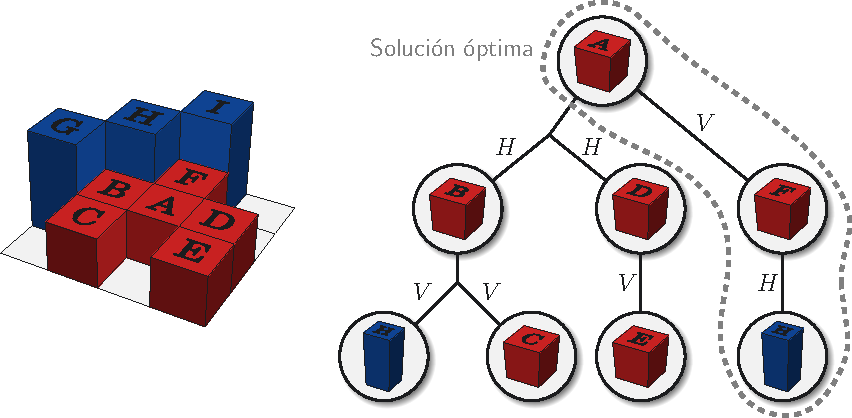
\includegraphics{arbol}%
\caption{Ejemplo de arreglo de objetos (izquierda) y el árbol de objetos-obstáculo correspondiente al cubo A (derecha). Como se puede observar, la solución óptima para tomar este cubo tiene costo 3.}%
\label{fig:arbol}%
\end{figure}
%
De acuerdo con las formas de sujeción establecidas, existen en general, dos secuencias distintas de objetos-obstáculo que hay que retirar de la malla para hacer sujetable a otro objeto particular. 
El costo $t_{ij}$ para tomar un objeto en la celda $e_{ij}$ es entonces la longitud de la secuencia con menos objetos a retirar, tal como se muestra en la Figura \ref{fig:arbol}, donde esta secuencia corresponde a la rama de menor longitud del árbol generado.
El cálculo de $t_{ij}$ se detalla en el Algoritmo \ref{alg:costo_individual}, el cual utiliza la Función \ref{fun:secuencia} recursiva.

La Función \ref{fun:secuencia} implementa un algoritmo de \textit{backtracking} para encontrar una de las secuencias de objetos-obstáculo para hacer sujetable y tomar un objeto de interés.
La secuencia encontrada por la función es considerada como solución al problema de hacer sujetable y tomar un objeto, esto debido a que él o los elementos al final de la secuencia siempre corresponderán a nodos hoja en el árbol de objetos-obstáculo del objeto de interés, como el que se muestra en Figura \ref{fig:arbol}.
Al retirar estos objetos, se harán sujetables los siguientes objetos de la secuencia y así sucesivamente hasta hacer sujetable al primer elemento de la secuencia, el cual corresponde al objeto que se desea tomar.

El algoritmo de \textit{backtracking} explora las ramas del árbol de objetos-obstáculo de un objeto particular y determina si al final de la rama existen objetos sujetables o no.
Si no es posible retirar ningún objeto de la rama en cuestión, la función falla.
Esto sucede cuando el elemento de la malla que se está analizando ya se encuentra agregado en la secuencia, lo cual puede ser indicativo de la existencia de un cuadro imposible en el arreglo.
Al fallar una función, todos sus procesos y los de las funciones en recursiones previas que la llamaron directa o indirectamente se invalidan, lo cual se traduce en que la secuencia que se había estado construyendo hasta ese momento sea descartada.
Después de esto se procede a explorar otra rama del árbol. 

La primera rama para la cual la función finalice con éxito es la que se toma como solución y cuyos objetos son añadidos a la secuencia considerada como resultado de la función.
%
\begin{center}
\begin{minipage}{0.90\textwidth}
\begin{function}[H]
	\BlankLine
	\Data{Celda $e_{ij}$ del objeto deseado y lista vacía $l$.}
	\QuarterBlankLine
	\Result{Lista $l$ con la secuencia de elementos a retirar.}
	\BlankLine
	\Definitions{
		\begin{definitions}[leftmargin=\leftmargin + \widthof{$o_{ij}$} + \labelsep]
			\item[$h_{ij}$] altura del elemento en la celda $e_{ij}$.
			\item[$o_{ij}$] \justify información de interés (clase y ubicación) del objeto en la celda $e_{ij}$ que será añadida a la secuencia.
		\end{definitions}
	}
	\BlankLine
	\Function{$\f{secuencia}(e_{ij},\: l)$}{%
	\BlankLine
		\lIf{$C_{ij} = C_0$}{Finalizar recursión con éxito.}
		\BlankLine
		\eIf{$o_{ij} \not\in l$}{
			\OneHalfBlankLine
			$\f{append}(o_{ij},\: l)$
			\OneHalfBlankLine
			\uIf{$\f{sujetable}(e_{ij})$}{
				\BlankLine
				Finalizar recursión con éxito.
				\HalfBlankLine
			}
			\SetArgSty{normaltext}
			\tcp*[l]{Ejecutar uno de los siguientes pares de recursiones:}
			\uElseIfWithNoThen{Par 1:}{
				\HalfBlankLine
				\lIf{$h_{i+1,\, j} \geq h_{ij}$}{$\f{secuencia}(e_{i+1,\, j},\: l)$}
				\lIf{$h_{i-1,\, j} \geq h_{ij}$}{$\f{secuencia}(e_{i-1,\, j},\: l)$}
				\HalfBlankLine
			}
			\uElseIfWithNoThen{Par 2:}{
				\HalfBlankLine
				\lIf{$h_{i,\, j+1} \geq h_{ij}$}{$\f{secuencia}(e_{i,\, j+1},\: l)$}
				\lIf{$h_{i,\, j-1} \geq h_{ij}$}{$\f{secuencia}(e_{i,\, j-1},\: l)$}
			}
			\Else{
				\tcp*[l]{Si en ambos pares alguna de las dos recursiones terminó con fallo:}
				Finalizar recursión con fallo (hacer \textit{backtracking} e intentar otra alternativa (par) de recursión).
				\HalfBlankLine		
			}
		}{
			\HalfBlankLine
			Finalizar recursión con fallo (hacer \textit{backtracking} e intentar otra alternativa (par) de recursión).
			\HalfBlankLine
		}%
		\HalfBlankLine
		Finalizar recursión con éxito.
		\QuarterBlankLine
	}%
	\caption{secuencia($e_{ij}$, $l$). Función de \textit{backtracking} para obtener una secuencia de objetos a retirar para hacer sujetable y tomar un objeto en la celda $e_{ij}$, el cual también se incluye al final de la secuencia.}%
	\label{fun:secuencia}%
\end{function}
\end{minipage}
\end{center}
%
A grandes rasgos, el funcionamiento del Algoritmo \ref{alg:costo_individual} consiste en explorar todas las ramas del árbol de objetos-obstáculo generado para un objeto de interés (como el mostrado en la Figura \ref{fig:arbol}), mediante la Función \ref{fun:secuencia}, encontrando todas sus soluciones posibles; esto es, todas las secuencias de objetos-obstáculo consideradas como solución.
El algoritmo cuenta los objetos-obstáculo de cada una de las secuencias y finalmente retorna la longitud de la rama más corta.
%
\begin{center}
\begin{minipage}{0.98\textwidth}
\begin{algorithm}[H]
	\OneHalfBlankLine
	\Data{Celda $e_{ij}$ del objeto deseado.}
	\Result{Costo $t_{ij}$ de tomar el objeto en $e_{ij}$.}
	\TwoBlankLines
	\tcp*[l]{Lista para almacenar todas las secuencias posibles para tomar un objeto.}
	$L = \{ \}$\;
	\TwoBlankLines
	\tcp*[l]{Función que retorna todas las soluciones posibles de $\f{secuencia()}$.}
	$\f{encontrarTodas}()$\;
	\TwoBlankLines
	$L = \f{encontrarTodas}(\f{secuencia}(e_{ij},\: l))$\;
	\TwoBlankLines
	$t_{ij} = \min\limits_i \left| L_i \right|$\;
	\HalfBlankLine
	\caption{Algoritmo para calcular el costo $t_{ij}$.}%
	\label{alg:costo_individual}%
\end{algorithm}
\end{minipage}
\end{center}
%
El costo global $T$, como se definió en la Sección \ref{sec:definiciones_y_consideraciones}, es simplemente la suma de los costos individuales $t_{ij}$:
%
\begin{equation}
T = \sum_{i,\hspace{1pt} j} \, t_{ij}
\end{equation}

\vspace{-\belowdisplayskip}%
%
%
\section{Algoritmo principal}
\label{sec:algoritmo_principal}
%
%
La aportación principal de este trabajo consiste en un algoritmo para el acomodo de objetos en un arreglo, que minimiza, en promedio, el costo posterior de acceso a ellos, esto es, minimiza el costo global $T$ previamente definido.
Dicho algoritmo, el cual adquiere sus fortalezas de todas las definiciones y condiciones precedentes, es un algoritmo de recocido simulado que utiliza a la función $\f{puntuacionGlobal}()$ como criterio de evaluación para encontrar un acomodo adecuado de los objetos, acorde a los fines establecidos.

La definición original del algoritmo de recocido simulado se puede encontrar en el artículo \cite{doi:10.1126/science.220.4598.671}, en el cual también se puede encontrar una implementación muy parecida a la realizada en este trabajo, la cual consiste en optimizar la longitud de cableado en la colocación de chips en una tarjeta de circuitos, modelándola como un arreglo en forma de malla 2D.

En el problema propuesto se plantean una serie de restricciones o reglas, las cuales deben ser cumplidas independientemente del método que se utilice para encontrar los acomodos de objetos óptimos.
Por ejemplo, una de las reglas básicas del problema, es que siempre se debe de respetar el número de objetos de cada clase que deben estar presentes en el arreglo final, retornado como solución.
Es a partir de este tipo de restricciones y reglas, así como de las libertades que en sí mismas se establecen, que se debe elegir una metodología de solución apropiada para el problema planteado.

Una estrategia de búsqueda razonable para encontrar un arreglo de objetos óptimo es partir de un acomodo arbitrario de objetos, el cual cumpla desde un inicio con la restricción descrita del número de objetos de cada clase en la malla y realizar cambios en este que, además de que estén orientados a mejorar el arreglo de acuerdo al criterio establecido, siempre mantengan de igual forma el número de los distintos objetos en la malla del arreglo anterior.
La clave del éxito de dicha estrategia de búsqueda dependerá de los criterios bajo los cuales se realicen dichos cambios y de cómo estos cumplirán con las restricciones del problema.
En este caso, el criterio principal para generar tales cambios es el sistema de puntuaciones propuesto.

Se eligió un algoritmo de recocido simulado para abordar el problema propuesto debido a que se adecúa muy bien a la búsqueda de vecindad planteada para este problema, la cual consiste en cambios graduales o mínimos en un arreglo dado, considerado como solución actual.
Dichos cambios graduales se refieren a los intercambios de pares de elementos en un arreglo, ya que, bajo las reglas establecidas, un intercambio de un par de elementos distintos en un arreglo se considera como el cambio mínimo necesario para hacerlo cambiar de estado, sin alterar el número de objetos de cada clase que hay en él.

Si bien puedieran existir mejores soluciones, al emplear otro tipo de algortimos o metodologías, el objetivo principal de este trabajo no es encontrar la solución más eficiente, sino encontrar o diseñar una solución aceptable al problema propuesto, del cual no parece haber antecedentes según la investigación realizada.
Se cree que, debido al nivel de simplificación y de condiciones particulares que requiere problema, encontrar el método de solución más eficiente no sería de mucha utilidad (más allá de la intelectual) en esta etapa, como si lo sería en etapas posteriores donde se pueda aplicar en situaciones reales.

No obstante, también se consideraron otros algoritmos y metodologías de búsqueda, de entre los cuales se eligió al recocido simulado por el balance entre la simpleza del método, su conocida eficiencia, además de la ya mencionada facilidad con la que se adapta a las reglas de búsqueda del problema propuesto.

Otros métodos de reconocido éxito fueron descartados al considerar que, o bien representaban un mayor costo computacional, o bien su metodología de búsqueda no se adecuaba a las características del problema.
Por ejemplo, en un algoritmo genético, se cree que los cambios en las instancias de arreglos serían más ``abruptos'' cuando se explora el espacio de búsqueda, debido a que en las recombinaciones de población se realizan muchos cambios para generar la descendencia, que pueden alejarse mucho de los arreglos padres y que, generalmente, no los mejoran en nuestro caso.
Además de que la condición en la que el número de elementos de cada clase en el arreglo se debe mantener de una recombinación a otra, es mucho más difícil de cumplir en un algoritmo genético.
Por lo cual, en dicho caso, se concluyó que no es la mejor manera de guiar la búsqueda hacia los arreglos óptimos.

En el Algoritmo \ref{alg:recocido_simulado} se presenta el algoritmo de recocido simulado utilizado.
%
\begin{center}
\begin{minipage}{0.98\textwidth}
\setlength{\interspacetitleruled}{5pt}
\begin{algorithm}[H]
	\OneQuarterBlankLine
	\Data{Temperatura inicial $T$, constantes $\alpha$, $a$, $b$, malla con objetos.}
	\HalfBlankLine
	\Result{Malla con objetos acomodados (representada por una matriz de enteros).}
	\TwoBlankLines
	%
	\tcp*[l]{Parámetros del algoritmo.}
	$T = \num{50000000}$\;
	$\mathrlap{\alpha}\hphantom{T} = 0.0000001$\;
	$\mathrlap{a}\hphantom{T} = 0.99991$\;
	$\mathrlap{b}\hphantom{T} = 1$\;
	\TwoBlankLines
	%
	\tcp*[l]{Puntajes actual y de intercambio.}
	$p_A =\, \f{puntuacionGlobal}()$\;
	$\mathrlap{p_I}\hphantom{p_A} =\, 0$\;
	\TwoBlankLines
	%
	\While{$T > \frac{b}{1 - a}$}{
		\OneHalfBlankLine
		Intercambiar aleatoriamente 2 elementos diferentes en la malla.\;
		\HalfBlankLine
		$p_I = \f{puntuacionGlobal}()$\;
		\BlankLine
		\eIf{$p_A \leq p_I$ \Or $\f{random}([0,1]) < e^{-\frac{{\scriptstyle p}_{\scriptscriptstyle A} -\, {\scriptstyle p}_{\scriptscriptstyle I}}{\alpha T}}$}{
			\HalfQuarterBlankLine
			Se acepta el intercambio.\;
			$p_A = p_I$
			\QuarterBlankLine
		}{
			\HalfBlankLine
			No se acepta el intercambio.
			\QuarterBlankLine
		}
		\BlankLine
		$T = aT + b$
		\QuarterBlankLine
	}%
	\HalfBlankLine
	\caption{Recocido simulado.}%
	\label{alg:recocido_simulado}%
\end{algorithm}
\end{minipage}
\end{center}
%
El algoritmo recibe como entrada principal una malla con los objetos acomodados de forma aleatoria. 
Después de inicializar los parámetros del algoritmo, tales como la temperatura, se inicia un proceso iterativo, en el cual, en primer lugar se calcula la puntuación global de la malla, para luego escoger dos elementos distintos en la malla de forma aleatoria e intercambiarlos de posición.
Dicho par de elementos puede ser un par \textsl{objeto~-objeto} o bien \textsl{objeto~-celda\! vacía}.
Al simular este intercambio se vuelve a calcular la puntuación global de la malla y esta se compara con la puntuación calculada antes de hacer el intercambio.
Si la puntuación después de hacer el intercambio es mejor, entonces el intercambio se acepta, de lo contrario la probabilidad de que se acepte disminuye considerablemente.
Este proceso de intercambios se repite hasta que se cumpla la condición de paro, la cual está relacionada con el decremento de la temperatura.
Finalmente, la salida del algoritmo será el acomodo encontrado.

Los parámetros iniciales mostrados en el Algoritmo \ref{alg:recocido_simulado} fueron los utilizados para generar los arreglos de mayor tamaño ($8\times 8$).
Para arreglos de menor tamaño estos parámetros se pueden relajar hasta cierto punto, sin sacrificar la calidad de los resultados.
El esquema de reducción de temperatura utilizado es el esquema aritmético-geométrico \cite{ouali2017performance}.

Si bien el proceso de ponderación de un arreglo se ideó con el fin de que el arreglo con mayor puntuación sea el óptimo, este podría no siempre ser el caso. 
Esto es debido a que existen algunos pocos casos especiales en los que, a causa de cómo están constituidas las reglas de puntuación, el algoritmo no le da la mejor puntuación al arreglo óptimo, sino a uno que tiene, en la mayoría de los casos donde se pudo corroborar, un costo global de una o dos acciones por encima del óptimo.
Estos casos especiales se pueden corregir mediante una extensión de las reglas de puntuación que considere las situaciones en las que ocurren, sin embargo, debido a que son muy poco frecuentes, se cree que la ganancia de extender las reglas es poca comparada con la complejidad añadida al modelo, por lo cual en esta ocasión no se considerará tal extensión.

Con la finalidad de evaluar el desempeño de dicho proceso de ponderación y del algoritmo propuesto, también se calculó el costo global real de los arreglos encontrados por el algoritmo propuesto, mediante el proceso descrito en la Sección \ref{subsec:costo}, el cual es un proceso exhaustivo.
Los costos globales de los arreglos encontrados por el algoritmo propuesto se compararon con los costos globales de los arreglos óptimos correspondientes, obtenidos mediante una búsqueda exhaustiva en lo casos donde fue posible realizarla. 
Los resultados de esta comparación se presentan en el siguiente capítulo.